\documentclass[a4paper,10pt]{article}
\usepackage[brazil]{babel}
\usepackage[utf8]{inputenc}
\usepackage[T1]{fontenc}
\usepackage{natbib}
\usepackage{graphicx}
\usepackage{url}

\title{IF796 Mineração na Web}
\author{Felipe Higino Paixão da Silva }

\begin{document}
\maketitle

\begin{figure}[h!]
    \centering
    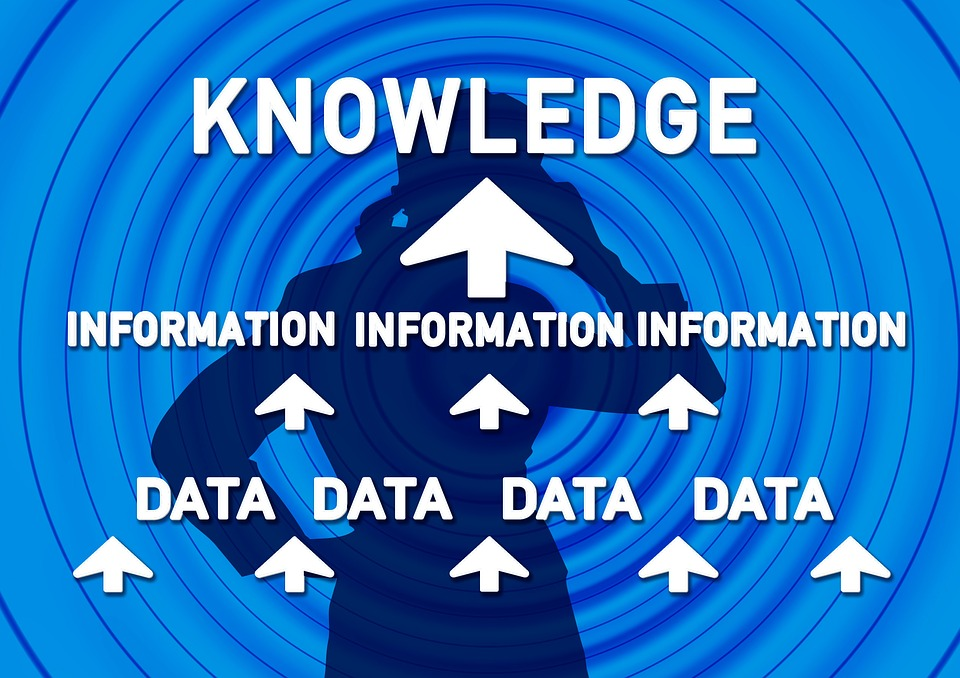
\includegraphics[scale = 0.2]{datato.jpg}
    \caption{\cite{img1}}
    \label{fig:my_label}
\end{figure}

%\center
%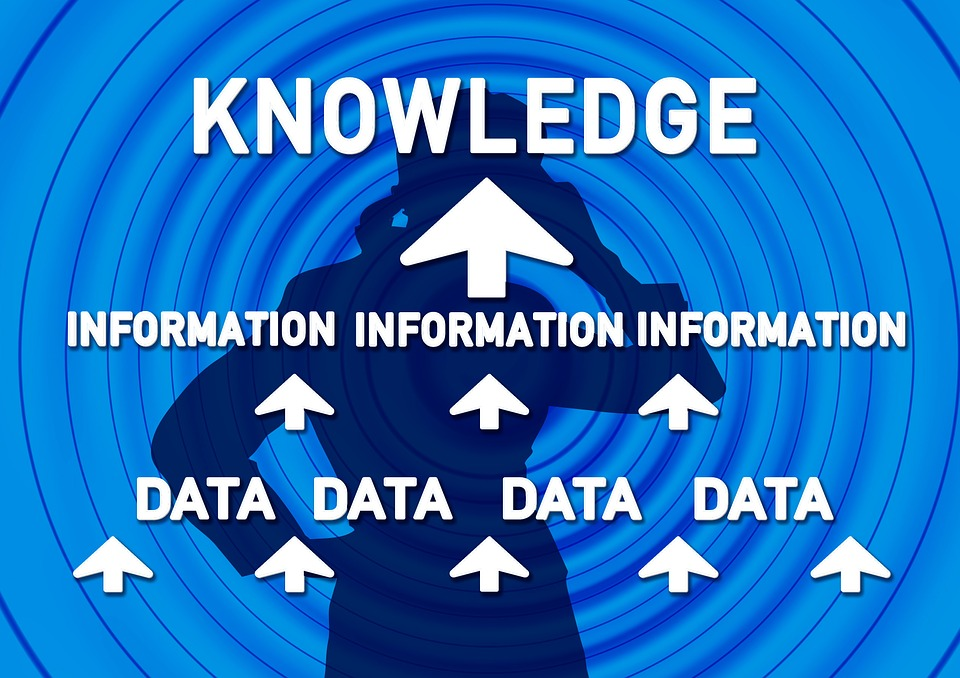
\includegraphics[scale = 0.2]{datato.jpg}\cite{img1}
%\flushleft

\section{Introdução}
"Informação de mais é tão ruim quanto informação nenhuma", esta máxima de W. H. Auden evidencia o problema do excesso de informação desorganizada, que, em certos momentos, pode se tornar tão desinformante quanto a própria falta de informação.

No mundo informatizado, com uma infinidade de informações sendo propagadas na internet, filtrar conteúdo não é uma tarefa simples, ao ponto de ser necessário um campo de estudos completo somente para realizar essa tarefa, eis que surge a Mineração na Web.

\section{Relevância}
A mineração na Web surge com o objetivo de amenizar o problema da "informação à deriva", modulando as informações em forma de documentos e categorizando-os, para uma consulta mais direta e eficiente no futuro.

A disciplina IF796 \citep{siteIF796} procura ensinar conceitos como: algorítimos de busca, Apresentação dos sistema RI (recuperação de informação) e mineração de texto, afim de possibilitar uma boa base de conhecimento prático e teórico acerca de mineração Web e recuperação de informação.

\begin{figure}
    \centering
    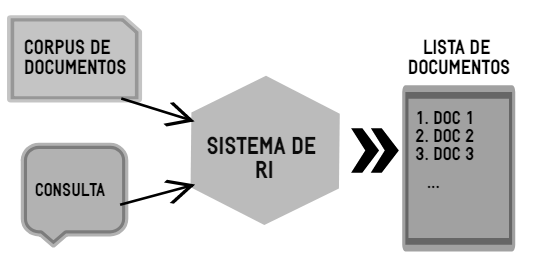
\includegraphics[scale = 0.5]{sistemaRI.PNG}
    \caption{Funcionamento da mineração de informação: Documentos são classificados pelas suas características, essas características são consultadas em um sistema centralizado RI que, por sua vez, retorna uma lista ordenada de documentos considerados relevantes pela consulta}
    \label{fig:my_label2}
\end{figure}


\section{Relação com outras disciplinas}
%TABELA DE COMPARAÇÃO
\begin{center}
\begin{tabular}{| p{4cm} | p{7cm} |}
\hline
NOME E CODIGO  & EXPLICAÇÃO                                                                    \\\hline
IF807 TOP. AVANC. SIST. SUP. DECIS. MIN. WEB\cite{perfilCurricular} & Técnicas avançadas e multidisciplinares da mineração web, voltado ao conhecimento científico e pesquisa     \\ \hline
IF672- ALGORITMOS E ESTRUTURAS DE DADOS\cite{AED} & Estruturas de dados, conceitos de grafos, ordenação e algorítmos de busca, fundamentais para o desenvolvimento de sistemas RI\\\hline
IF678- INFRA-ESTRUTURA DE COMUNICACAO\cite{IEC}   & Transporte de informações pela rede, transmissão de dados \\ \hline
IF684- SISTEMAS INTELIGENTES\cite{perfilCurricular}   &  Tópicos sobre busca e aprendizagem de máquina presentes em algorítmos de busca (RI) como Google e Yahoo \\ \hline
\end{tabular}
\end{center}

\bibliographystyle{plain}
\bibliography{fhps}
\end{document}